\documentclass[10pt, letter, twocolumn]{article}

\usepackage{times} % Times New Roman Font
\usepackage{newtxtext} % Use Times New Roman for text
\usepackage{newtxmath} % Use Times New Roman for math

\usepackage{stfloats}
\usepackage{geometry}
\usepackage{setspace}
\usepackage{titlesec}
\usepackage{caption}
\usepackage{authblk}
\usepackage[hidelinks]{hyperref}
\usepackage{booktabs} % For better table lines
\usepackage{xcolor}   % specify colors by name (e.g. "red")
\usepackage{ulem}   % For underlining % fancy underlines
\usepackage{tabularx} % advanced tables
\usepackage{graphicx} % Required for including images
\usepackage{float}    % Required for the [H] option

\usepackage[skip=5pt]{parskip} % don't indent paragraphs
% Set the font size for figure captions
\captionsetup{font={small}} % Set caption font size to 9pt
\usepackage[labelfont=bf,belowskip=0pt,aboveskip=5pt]{caption} % Makes figure labels bold

% Define a custom blue color
\definecolor{WordBlue}{RGB}{26,92,189}

% Set the margins
\geometry{
    top=20mm,
    left=15mm,
    right=15mm,
    bottom=25mm,
}
%% Bibliography configuration
\usepackage[backend=biber, style=numeric, sorting=none]{biblatex}

\DeclareFieldFormat{title}{\textit{#1}} % Italicize titles
\DeclareFieldFormat{title}{\textit{#1}}
\DeclareFieldFormat{journaltitle}{\textit{#1}}
\DeclareFieldFormat{year}{(#1)}
\DeclareFieldFormat{pages}{#1}

% Define a new bibliography driver for articles
\DeclareBibliographyDriver{article}{%
  \printnames{author}%
  \addspace\printfield{year}.%
  \addspace\printfield{journaltitle},%
  \addspace \textbf{\printfield{volume}}:%
  \addspace \printfield{pages}.%
}

% Define a new bibliography driver for books
\DeclareBibliographyDriver{book}{%
  \printnames{author}.%
  \addspace\printfield{year}%
  \addspace\printfield{title};%
  \addspace\printlist{publisher}.
}

\addbibresource{bibliography.bib} %Import the bibliography file

% Formatting configuration

% Disable hyphenation
\hyphenpenalty=10000
\exhyphenpenalty=10000

% Set the column width
\setlength{\columnsep}{30pt}
\setlength{\columnwidth}{86mm}

% Adjust spacing
\setlength{\textfloatsep}{0pt} % Space between a float at the top/bottom and the text
\setlength{\intextsep}{2pt}    % Space above and below in-text floats

% Set the font size for section headings
\titleformat{\section}{\normalfont\normalsize\bfseries}{\thesection}{1em}{}

% Set spacing before and after section headers
% \titlespacing{\section}{0pt}{12pt plus 0pt minus 0pt}{10pt plus 0pt minus 0pt} % {left}{before}{after}
\titlespacing*%
    {\section}% 
    {0pt}% {left}
    {1em plus 0pt minus 0pt}% {before}
    {0.5em plus 0pt minus 0pt}%{after}

% Define custom title command
\makeatletter
    \def\@maketitle{
  \begin{center}
    {\normalsize\textbf{\@title} \par}%
    \vskip 1.0em
    {\large
      \lineskip 0.5em
      \begin{tabular}[t]{c}%
        \@author
      \end{tabular}\par}
  \end{center}%
  \vskip 1.5em}
\makeatother

% Adjust spacing for author affiliations
\renewcommand\Authfont{\normalsize} % Set author font size to 10pt
\renewcommand\Affilfont{\normalsize} % Set affiliation font size to 10pt
\setlength{\affilsep}{0pt} % Remove extra space between authors and affiliations

\title{Abstract Template for ISB2025 in Stockholm} 
\author[1,2]{\textbf{First I. Author}}
\author[1,2]{Second I. Author}
\author[3]{Third I. Author}
\affil[1]{BMC Laboratory, The Swedish School of Sport and Health Sciences, Stockholm, Sweden}
\affil[2]{KTH MoveAbility Lab, Dept. Engineering Mechanics, KTH Royal Institute of Technology, Stockholm, Sweden}
\affil[3]{CLINTEC Institution, Karolinska Institute, Stockholm, Sweden}
\affil[ ]{Email: \href{mailto:corresponding.author@institution.se}{\textcolor{WordBlue}{\uline{corresponding.author@institution.se}}}} % Mailto link

\begin{document}
\maketitle

% Remove page numbers
\thispagestyle{empty}

% Center values within the cells
\newcolumntype{Y}{>{\centering\arraybackslash}X}
\begin{table*}[b]
    \centering
    \caption{Interesting data from well-executed experiments. The data have been arranged in an interesting and clear manner.}
    \begin{tabularx}{\linewidth}{|X|Y|Y|Y|Y|Y|Y|Y|Y|Y|} % One left-aligned column and six centered columns
        \hline
        Data & 234 & 243 & 210 & 2323 & 443 & 3432 & 234 & 3223 & 2423 \\ % Data row
        \hline
        Other & 234 & 234 & 233 & 2323 & 3243 & 4342 & 2342 & 234 & 342 \\ % Other row
        \hline
    \end{tabularx}
    \label{tab:table-1}
\end{table*}
\section*{Summary}
A summary (150 words maximum, plain text) should be included as the first section. The text of the summary should also be copied and pasted separately into the dedicated field within the online abstract submission system at the time of abstract submission. This summary will appear in the on-line program.

\section*{Introduction}

This document serves as an abstract template and contains information about the abstract submission process. All abstracts must be submitted electronically via the official website of ISB2025, by the deadline indicated. 

The abstract should be prepared using this template and submitted as a PDF file of $\leq$ 5 MB. The congress organizers reserve the right to reject abstracts that do not adhere to this template.

\section*{Methods}
The abstract is limited to one A4 size page (210 × 297 mm 8.27 in × 11.69 in), with two columns of text. The top margin should be 20 mm, while left, right and bottom margins should be 15 mm. The column width should be 86 mm. All text should be in font Times New Roman or Times, size 10 pt, except for the figure/table captions, which should be in size 9 pt.

The title (boldface), authors, and author affiliations should be centered across the top of the page. Use numerical superscripts to distinguish authors who are from different institutions. An email address of the corresponding author must be included. The \textbf{presenting author} should be in bold.

The text within each column should be right- and left-justified, without paragraph indentations. The body of the manuscript should be divided into sections such as Introduction, Methods, Results and Discussion, Conclusions (all words capitalized and bold). Spacing (already set in this template): single-spaced, 5 pt for the text, 10 pt before and 5 pt after for the section headers.

\section*{Results and Discussion}
A maximum of two items, figures and/or tables are recommended within the document. The figures or tables (if included) should be placed immediately after a paragraph and should be referenced parenthetically in the text (Figure \ref{fig:expected-abstracts}). Captions should be placed below each figure and above each table. Tables may extend across two columns when needed, in which case they must be placed at the bottom of the page (Table \ref{tab:table-1}). In Microsoft Word, use “Layout $\rightarrow$ Columns” to control which parts of the text are in single column format.
\begin{figure}[H]
    \centering
    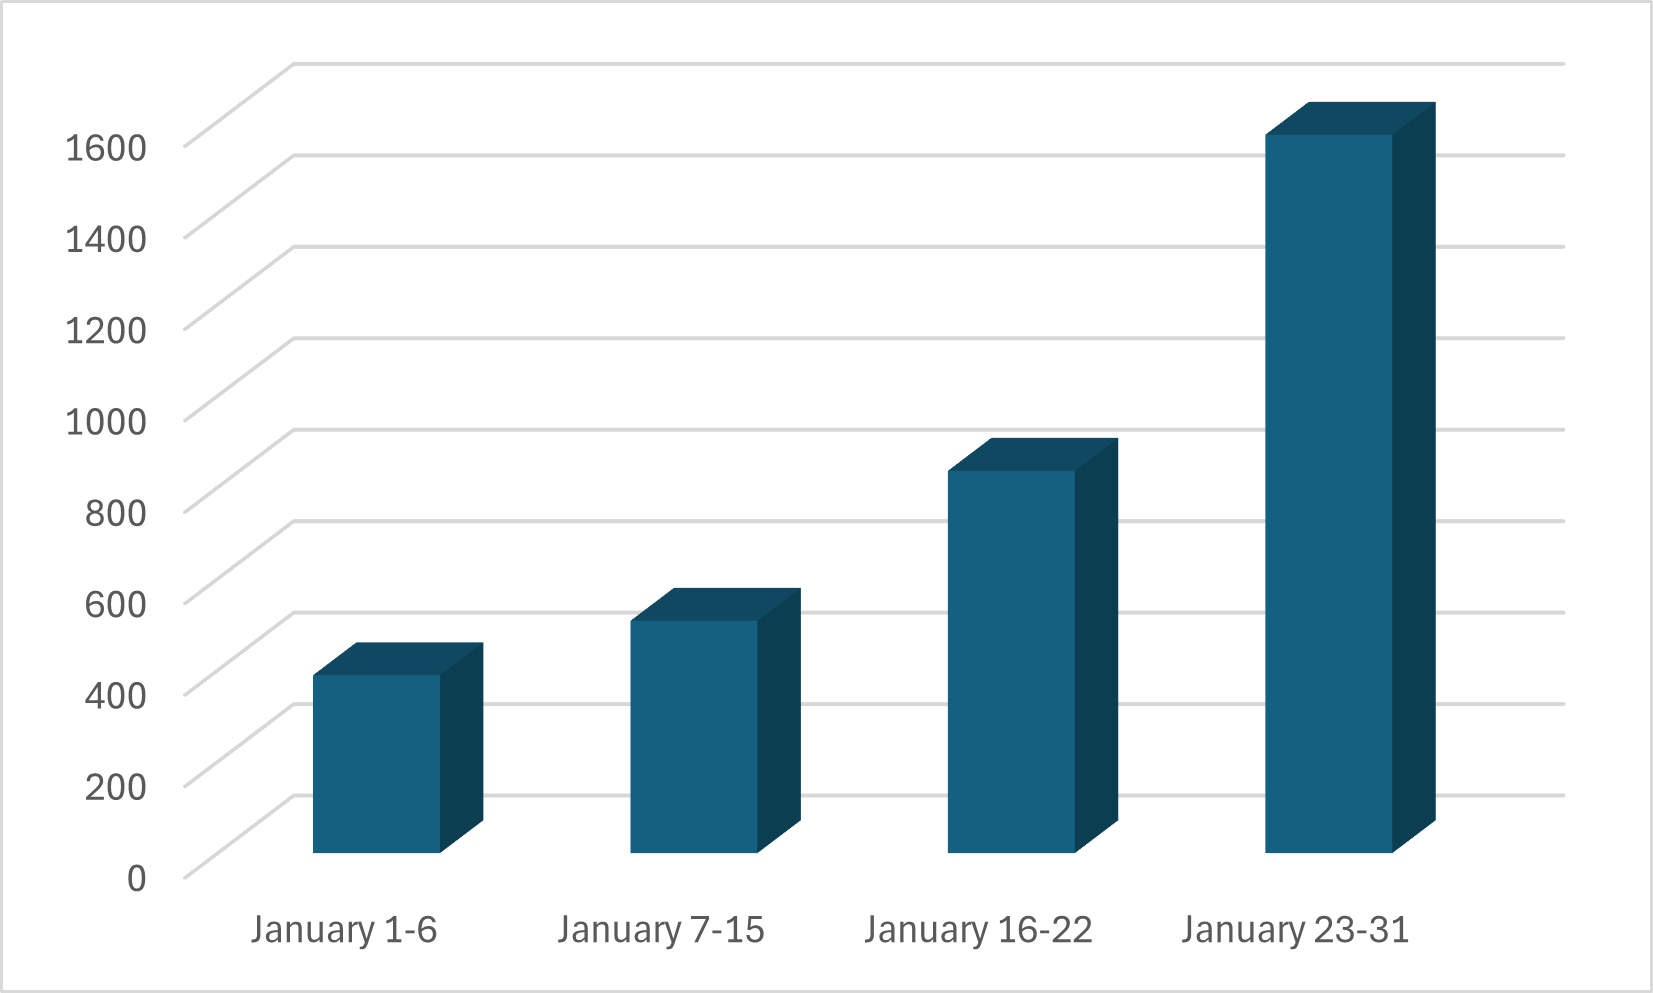
\includegraphics[width=\linewidth]{isb-figure.png} % Placeholder box
    \caption{Expected abstracts for ISB2025 in January 2025.}
    \label{fig:expected-abstracts}
\end{figure}
Reference citations within the text are to be made with numbers in square brackets \cite{author2023, someauthor2023}. References are to be formatted as illustrated below. Place the journal or book title in \textit{Italics}, with volume numbers in \textbf{bold} \cite{author2023b}. 

\section*{Conclusions}

If an incomplete submission is received, it may be withheld from acceptance until the authors supply all required components.

\section*{Acknowledgments}
Acknowledgments are optional and should specify research funding and resources including organization name and reference numbers (if applicable).

\printbibliography %Prints bibliography

\end{document}